\stepcounter{footnote}
\footnotetext{\label{SEEDfootnote:tie-braking}Depending on how the \A~algorithm
handles tie-braking, different sets of states could be explored. For simplicity,
we show all states that \emph{could potentially} be explored.}
\begin{figure}[t]
    \centering
	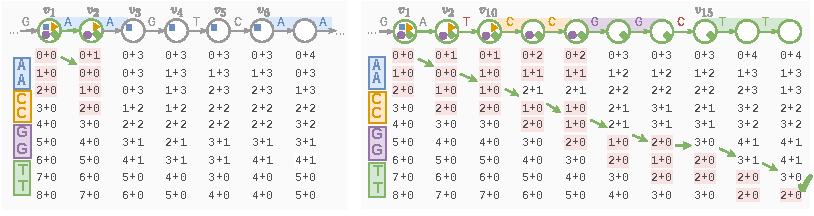
\includegraphics[width=\linewidth]{figures/seed-heuristic-tables}
	\caption{Exploration of $\AG[q]$, searching for a shortest path from the
	first to the last row using the \seedh. The table entry in the $i^\text{th}$
	row (zero indexed) below node $v$ shows $g\st{v}{i}+h\st{v}{i}$, where
	$g\st{v}{i}$ is the shortest distance from any starting state $\st{u}{0}$ to
	$\st{v}{i}$.
	%
	States that may\textsuperscript{\cref{SEEDfootnote:tie-braking}} be expanded by
	the \A~algorithm are highlighted in \colorbox{pink-highlight}{pink}, and the
	rest of the states are shown for completeness even though they are never
	expanded. The shortest path corresponding to the best alignment is shown
	with green arrows~(\textcolor{dark-green}{$\pmb{\rightarrow}$}).}
	%
	\label{SEEDfig:exploration-table}
\end{figure}
